\section{Multifaceted Mode-I Convergence Evaluation}
\label{sec:multifaceted_convergence}

In accordance with supervisor directives, mesh adequacy and numerical convergence are evaluated across multiple complementary physical and energetic quantities rather than peak reaction force alone.

\subsection{Spatial Mesh Resolution Series ($S_1$--$S_4$)}
Four uniform meshes spanning element edge lengths from $h = 3.0\,\mu\mathrm{m}$ ($S_1$, $15{,}192$ elements) down to $h = 1.25\,\mu\mathrm{m}$ ($S_4$, $51{,}408$ elements) evaluate spatial discretization characteristics ($h/l_0 \in [0.167, 0.400]$ at fixed $l_0 = 7.5\,\mu\mathrm{m}$), alongside a separate historical fine-mesh result ($h = 1.0\,\mu\mathrm{m}$, $69{,}384$ elements, Job \texttt{1406019.mmaster02}):
\begin{enumerate}
  \item \textbf{Initial Structural Stiffness $K_0$ is Stable:} Across the governed $S_1$--$S_4$ spatial series, $K_0$ varies from $137.945520$ to $137.841200\,\mathrm{kN/mm}$. An additional historical $h=1.0\,\mu\mathrm{m}$ mesh gives $137.823301\,\mathrm{kN/mm}$, confirming that the initial structural stiffness remains exceptionally stable over the broader tested resolution range ($< 0.09\%$ total variation, $R^2 > 0.999999$). Classified as \textbf{\texttt{CONVERGED / STABLE}}.
  \item \textbf{Peak Force $F_{\max}$ and Displacement $u_{\mathrm{peak}}$ are Mesh-Sensitive:} Across the full tested range, peak force decreases monotonically from $0.7578\,\mathrm{kN}$ ($S_1$) to $0.7255\,\mathrm{kN}$ (historical fine mesh), a total reduction of $4.26\%$ (Fig.~\ref{fig:spatial_fu_pack} and \ref{fig:spatial_metrics_pack}). The displacement at peak load shifts from $5.857$ to $5.575\,\mu\mathrm{m}$, corresponding to an approximately $4.81\%$ earlier peak with refinement. Classified as \textbf{\texttt{MESH-SENSITIVE}}.
\end{enumerate}

\begin{figure}[htbp]
  \centering
  \includegraphics[width=0.82\textwidth]{fig_mode1_spatial_fu_convergence.pdf}
  \caption{Mode-I tensile force-displacement response across uniform mesh resolutions ($S_1$--$S_4$ plus historical fine mesh), showing identical elastic stiffness and systematic peak load mesh sensitivity.}
  \label{fig:spatial_fu_pack}
  \figureconclusion{The elastic slopes are effectively mesh-independent, but refinement systematically lowers $F_{\max}$ and shifts $u_{\mathrm{peak}}$ earlier. Elastic response is stable; fracture initiation remains spatially mesh-sensitive.}
\end{figure}

\begin{figure}[htbp]
  \centering
  \includegraphics[width=0.92\textwidth]{fig_mode1_spatial_convergence_metrics.pdf}
  \caption{Discretization ratio ($h/l_0$) scaling metrics: (a) exceptional invariance of initial stiffness $K_0$ ($\Delta < 0.09\%$); (b) monotonic mesh sensitivity of peak force $F_{\max}$ ($4.26\%$); (c) peak displacement shift $u_{\mathrm{peak}}$; (d) matched-displacement external work $W_{\mathrm{trap}}$.}
  \label{fig:spatial_metrics_pack}
  \figureconclusion{Convergence is quantity-dependent: $K_0$ and matched pre-peak work are nearly invariant, whereas $F_{\max}$ and $u_{\mathrm{peak}}$ change systematically with $h/l_0$. The solution must not be described as fully mesh-converged.}
\end{figure}

\clearpage

\subsection{Temporal Time-Increment Scaling ($T_1$--$T_3$)}
Time incrementation was tested across three schedules at fixed baseline resolution ($h = 3.0\,\mu\mathrm{m}$): Case $T_1$ (coarse $2\times$, $3{,}500$ incs), Case $T_2$ (nominal $1\times$, $7{,}000$ incs), and Case $T_3$ (fine $0.5\times$, Job \texttt{1406317.mmaster02}, completed all $10{,}022$ Step-2 incs to $u = 10.0\,\mu\mathrm{m}$).
\begin{itemize}
  \item \textbf{Peak Mechanical Invariance:} Initial stiffness $K_0$ varies by $<0.001\%$, and peak force varies by $<0.07\%$ ($0.75815 \to 0.75763\,\mathrm{kN}$), proving temporal stability of limit loads (\textbf{\texttt{CONVERGED / STABLE}}, Fig.~\ref{fig:temporal_pack}).
  \item \textbf{Energetic Temporal Sensitivity:} Terminal trapezoidal boundary work $W_{\mathrm{trap}}$ varies by $3.24\%$ ($2.41011 \to 2.33189\,\mathrm{mJ}$), and the two-term bookkeeping difference $\mathcal{R}_{\mathrm{bookkeeping}} = W_{\mathrm{trap}} - (E_{\mathrm{elas}} + E_{\mathrm{frac}})$ shifts from $+0.378\%$ to $+3.541\%$ (\textbf{\texttt{TEMPORALLY SENSITIVE}}).
\end{itemize}

\begin{figure}[htbp]
  \centering
  \includegraphics[width=0.78\textwidth]{fig_mode1_temporal_convergence.pdf}
  \caption{Mode-I temporal convergence across time increment scales ($T_1$: $2\times$, $T_2$: $1\times$, $T_3$: $0.5\times$, Job \texttt{1406317.mmaster02}), showing step-size invariance of the mechanical peak.}
  \label{fig:temporal_pack}
  \figureconclusion{The mechanical response through the peak is temporally converged over $T_1$--$T_3$ ($\Delta K_0<0.001\%$, $\Delta F_{\max}<0.07\%$). The spatial peak sensitivity in Fig.~\ref{fig:spatial_fu_pack} therefore cannot reasonably be attributed to insufficient time resolution; post-peak energy is assessed separately.}
\end{figure}

\clearpage

\subsection{Adaptive Mesh Temporal Refinement Audit ($2\times$ Refinement: Job 1410027 vs 1409982)}
\label{sec:adaptive_temporal_refinement_audit}

To evaluate time-step convergence on the production $14{,}483$-element adaptive mesh, a controlled $2\times$ temporal refinement diagnostic (Job \texttt{1410027.mmaster02}, $8{,}958$ completed increments, Package~26) was audited against the baseline canonical ET1 solve (Job \texttt{1409982.mmaster02}, $4{,}890$ increments, Package~25). All physical parameters, 3-layer UEL subroutine source (\texttt{CE8D5EDC...}), and solver controls ($I_A=10, \Delta t_{\min}=10^{-9}\,\mathrm{s}$) were kept strictly invariant.

\begin{enumerate}
  \item \textbf{Elastic and Pre-Peak Temporal Stability:}
  \begin{itemize}
    \item \textbf{Canonical Stiffness $K_0$ ($u \le 1.0\,\mu\mathrm{m}$):} Baseline $K_0 = 137.909558\,\mathrm{kN/mm}$ ($N=400$, $\Delta u = 2.50\,\mathrm{nm}$) vs $2\times$ Refined $K_0 = 137.909975\,\mathrm{kN/mm}$ ($N=800$, $\Delta u = 1.25\,\mathrm{nm}$), yielding $\Delta K_0 = \mathbf{+0.000302\%}$ ($R^2 = 0.99999960$). Classified as \textbf{\texttt{TEMPORALLY\_STABLE}}.
    \item \textbf{Peak Reaction Force $F_{\max}$ ($u \approx 5.73\,\mu\mathrm{m}$):} Baseline $F_{\max} = 0.743701\,\mathrm{kN}$ ($u_{\mathrm{peak}} = 5.733\,\mu\mathrm{m}$) vs $2\times$ Refined $F_{\max} = 0.743530\,\mathrm{kN}$ ($u_{\mathrm{peak}} = 5.730\,\mu\mathrm{m}$), yielding $\Delta F_{\max} = \mathbf{-0.0229\%}$ and $\Delta u_{\mathrm{peak}} = \mathbf{-0.052\%}$. Classified as \textbf{\texttt{TEMPORALLY\_STABLE}}.
    \item \textbf{Pre-Peak Matched Parity:} Pointwise force discrepancy across all reached pre-peak states ($u \in [1.0, 5.733]\,\mu\mathrm{m}$) is bounded by $|\Delta F|/F \le \mathbf{0.0436\%}$ (Fig.~\ref{fig:t2x_fu_audit} and \ref{fig:t2x_discrepancy_audit}).
  \end{itemize}

  \item \textbf{Energy Partitioning Dynamics at Peak:}
  Total model energy $E_{\mathrm{model}} = E_{\mathrm{elas}} + E_{\mathrm{frac}}$ at peak displacement ($u = 5.730\,\mu\mathrm{m}$) is $2.205225\,\mathrm{mJ}$ in both models ($\Delta E_{\mathrm{model}} = \mathbf{0.000000\,\mathrm{mJ}}$ to 6 decimal places, Fig.~\ref{fig:t2x_energy_audit}).

  \item \textbf{Common Displacement Interval \& Zero Forward-Filling:}
  The common actually reached displacement domain is $u \in [0.0, 7.46970\,\mu\mathrm{m}]$. Unreached states ($u > 7.46970\,\mu\mathrm{m}$) are strictly classified as \textbf{\texttt{NOT\_REACHED}} with zero forward-filling.

  \item \textbf{Post-Fracture Severed-Wake Solver Stagnation Mechanism:}
  Both models experienced cutback ceiling exhaustion ($I_A=10$) down to $\Delta t_{\min} = 10^{-9}\,\mathrm{s}$ in the severed wake ($x \approx 0.56\,\mathrm{mm}, d \approx 0.999, \sigma \approx 0$). In the refined model, halving the nominal increment scale ($\Delta u_{\mathrm{nom}} = 0.50\,\mathrm{nm}$ vs $1.00\,\mathrm{nm}$) halved $\Delta u_{\mathrm{inc}}$, making the dimensionless displacement correction check $c_{\max} / \Delta u_{\mathrm{inc}}$ twice as strict, triggering cutback exhaustion at $u = 7.470\,\mu\mathrm{m}$ instead of $7.889\,\mu\mathrm{m}$ (Fig.~\ref{fig:t2x_telemetry_audit}). Classified as \textbf{\texttt{POST\_FRACTURE\_CONVERGENCE\_NORMALIZATION\_SENSITIVITY\_VERIFIED}} and \textbf{\texttt{TEMPORALLY\_SENSITIVE\_POSTPEAK}}.
\end{enumerate}

\begin{figure}[htbp]
  \centering
  \includegraphics[width=0.82\textwidth]{fig_mode1_stage14_temporal_convergence_fu.pdf}
  \caption{Mode-I adaptive mesh $2\times$ temporal refinement audit: $F$--$u$ response comparing Baseline ($4{,}890$ incs, $u_{\mathrm{term}}=7.889\,\mu\mathrm{m}$) against $2\times$ Refined ($8{,}958$ incs, $u_{\mathrm{term}}=7.470\,\mu\mathrm{m}$), highlighting common reached interval and pre-peak $K_0$ inset.}
  \label{fig:t2x_fu_audit}
  \figureconclusion{Pre-peak mechanical response and peak load are fully temporally converged ($\Delta K_0 = +0.00030\%$, $\Delta F_{\max} = -0.0229\%$). The earlier termination at $u = 7.470\,\mu\mathrm{m}$ is a post-fracture wake normalization artifact, not physical instability.}
\end{figure}

\begin{figure}[htbp]
  \centering
  \includegraphics[width=0.82\textwidth]{fig_mode1_stage14_temporal_discrepancy.pdf}
  \caption{Pointwise force discrepancy $\Delta F$ and relative difference [\%] over the common reached displacement interval $u \in [0, 7.470]\,\mu\mathrm{m}$, separating elastic ($\le 0.0436\%$) from post-peak broken-state regimes.}
  \label{fig:t2x_discrepancy_audit}
  \figureconclusion{Discrepancy is negligible in the elastic regime ($<0.01\,\mathrm{N}$), tight across peak load ($0.32\,\mathrm{N}$), and settles onto a minute post-fracture wake offset ($0.7\text{--}0.8\,\mathrm{N}$) in the fully severed ligament.}
\end{figure}

\begin{figure}[htbp]
  \centering
  \includegraphics[width=0.92\textwidth]{fig_mode1_stage14_temporal_energy_evolution.pdf}
  \caption{Matched energy evolution for baseline and $2\times$ temporal refined models: (a) stored elastic energy $E_{\mathrm{elas}}$ and fracture functional $E_{\mathrm{frac}}$; (b) total model energy $E_{\mathrm{model}}$ and external work $W_{\mathrm{ext}}$.}
  \label{fig:t2x_energy_audit}
  \figureconclusion{Energy partitioning is bitwise identical through elastic loading and matches to $0.000000\,\mathrm{mJ}$ at peak load ($2.205225\,\mathrm{mJ}$). Broken-state fracture dissipation converges within $2.98\%$.}
\end{figure}

\begin{figure}[htbp]
  \centering
  \includegraphics[width=0.82\textwidth]{fig_mode1_stage14_temporal_solver_telemetry.pdf}
  \caption{Solver time increment $\Delta t$ progression (log scale) and Newton equilibrium iterations per increment across baseline and $2\times$ refined runs, showing consistent 3 iters/inc across all reached states.}
  \label{fig:t2x_telemetry_audit}
  \figureconclusion{Both simulations advance with steady 3 Newton iterations per increment throughout linear and softening phases, demonstrating zero iterative degradation prior to wake cutback exhaustion.}
\end{figure}

\clearpage

\subsection{Adaptive Remeshing Series ($A_1$--$A_4$)}
Figure~\ref{fig:adaptive_meshes_comparison_pack} displays the Abaqus-native adaptive meshes generated using `errorTarget` values of $1\%$, $2\%$, $3\%$, and $5\%$ ($A_1$--$A_4$), showing the full specimen domain and crack-tip zoom windows. As target discretization tolerance relaxes, element density smoothly transitions from intense crack-line refinement ($71{,}320$ elements) down to coarser background meshes ($4{,}194$ elements).

\begin{figure}[htbp]
  \centering
  \includegraphics[width=0.98\textwidth]{fig_adaptive_meshes_comparison.pdf}
  \caption{Abaqus-native adaptive meshes generated for the Mode-I benchmark using \texttt{errorTarget} values of (a) 1\%, (b) 2\%, (c) 3\%, and (d) 5\%. The corresponding production meshes contain $71{,}320$, $15{,}396$, $7{,}633$, and $4{,}194$ underlying finite elements, respectively. Full-domain views and identical crack-tip zooms illustrate how relaxing the target error changes the spatial refinement distribution.}
  \label{fig:adaptive_meshes_comparison_pack}
  \figureconclusion{Relaxing \texttt{errorTarget} from $1\%$ to $5\%$ sharply reduces element count and progressively coarsens the crack-tip region, exposing the intended accuracy--cost trade-off of native error-controlled pre-refinement.}
\end{figure}

Figure~\ref{fig:adaptive_pack} shows the corresponding force--displacement response:
\begin{itemize}
  \item \textbf{Elastic Agreement:} All adaptive models reproduce the canonical initial stiffness $K_0 \approx 137.85\,\mathrm{kN/mm}$ within $0.09\%$.
  \item \textbf{Softening Response:} $A_1$ follows the reference softening drop up to cutback at $u = 6.77\,\mu\mathrm{m}$, while coarser meshes ($A_2$--$A_4$) reach the full $10.0\,\mu\mathrm{m}$ endpoint. Mesh $A_4$ exhibits an elevated post-peak plateau ($F \sim 0.033\,\mathrm{kN}$), classified as \textbf{\texttt{OBSERVED\_FORCE\_PLATEAU (CRACK-PINNING HYPOTHESIS / NOT YET INDEPENDENTLY PROVEN)}}.
\end{itemize}

\begin{figure}[htbp]
  \centering
  \includegraphics[width=0.98\textwidth]{fig_mode1_adaptive_convergence.pdf}
  \caption{Force--displacement response of the canonical uniform reference $S_1$ and native adaptive meshes $A_1$--$A_4$: (a) full response over $u \in [0, 10]\,\mu\mathrm{m}$; (b) post-peak zoom over $u \in [5.4, 10]\,\mu\mathrm{m}$. Production adaptive meshes contain $71{,}320$, $15{,}396$, $7{,}633$, and $4{,}194$ underlying finite elements for \texttt{errorTarget} values of 1\%, 2\%, 3\%, and 5\%, respectively. $A_1$ terminates at $u = 6.77\,\mu\mathrm{m}$, whereas $A_2$--$A_4$ reach $10\,\mu\mathrm{m}$.}
  \label{fig:adaptive_pack}
  \figureconclusion{All adaptive meshes recover the elastic stiffness, yet their initiation and post-peak responses separate substantially. Matching $K_0$ is therefore insufficient to establish fracture adequacy, and $A_1$--$A_4$ are not adaptive-tolerance-independent post peak; the $A_4$ plateau mechanism remains unproven.}
\end{figure}

\clearpage

\subsection{Phase-Field Contours, Crack Symmetry, and Localization Profiles}
Figures~\ref{fig:matched_contours_pack}--\ref{fig:path_dev_pack} separate three questions: where the crack propagates, how its centerline evolves, and how wide the diffuse localization band remains. Pre-peak profiles agree closely; near and after the peak, propagation timing and extent become resolution-dependent. Across all fixed and adaptive meshes, the centroid remains within $3.10\,\mu\mathrm{m}$ of the Mode-I symmetry line, whereas the $d\ge0.50$ band retains a resolution-sensitive full width of approximately $20$--$30\,\mu\mathrm{m}$.

\begin{figure}[htbp]
  \centering
  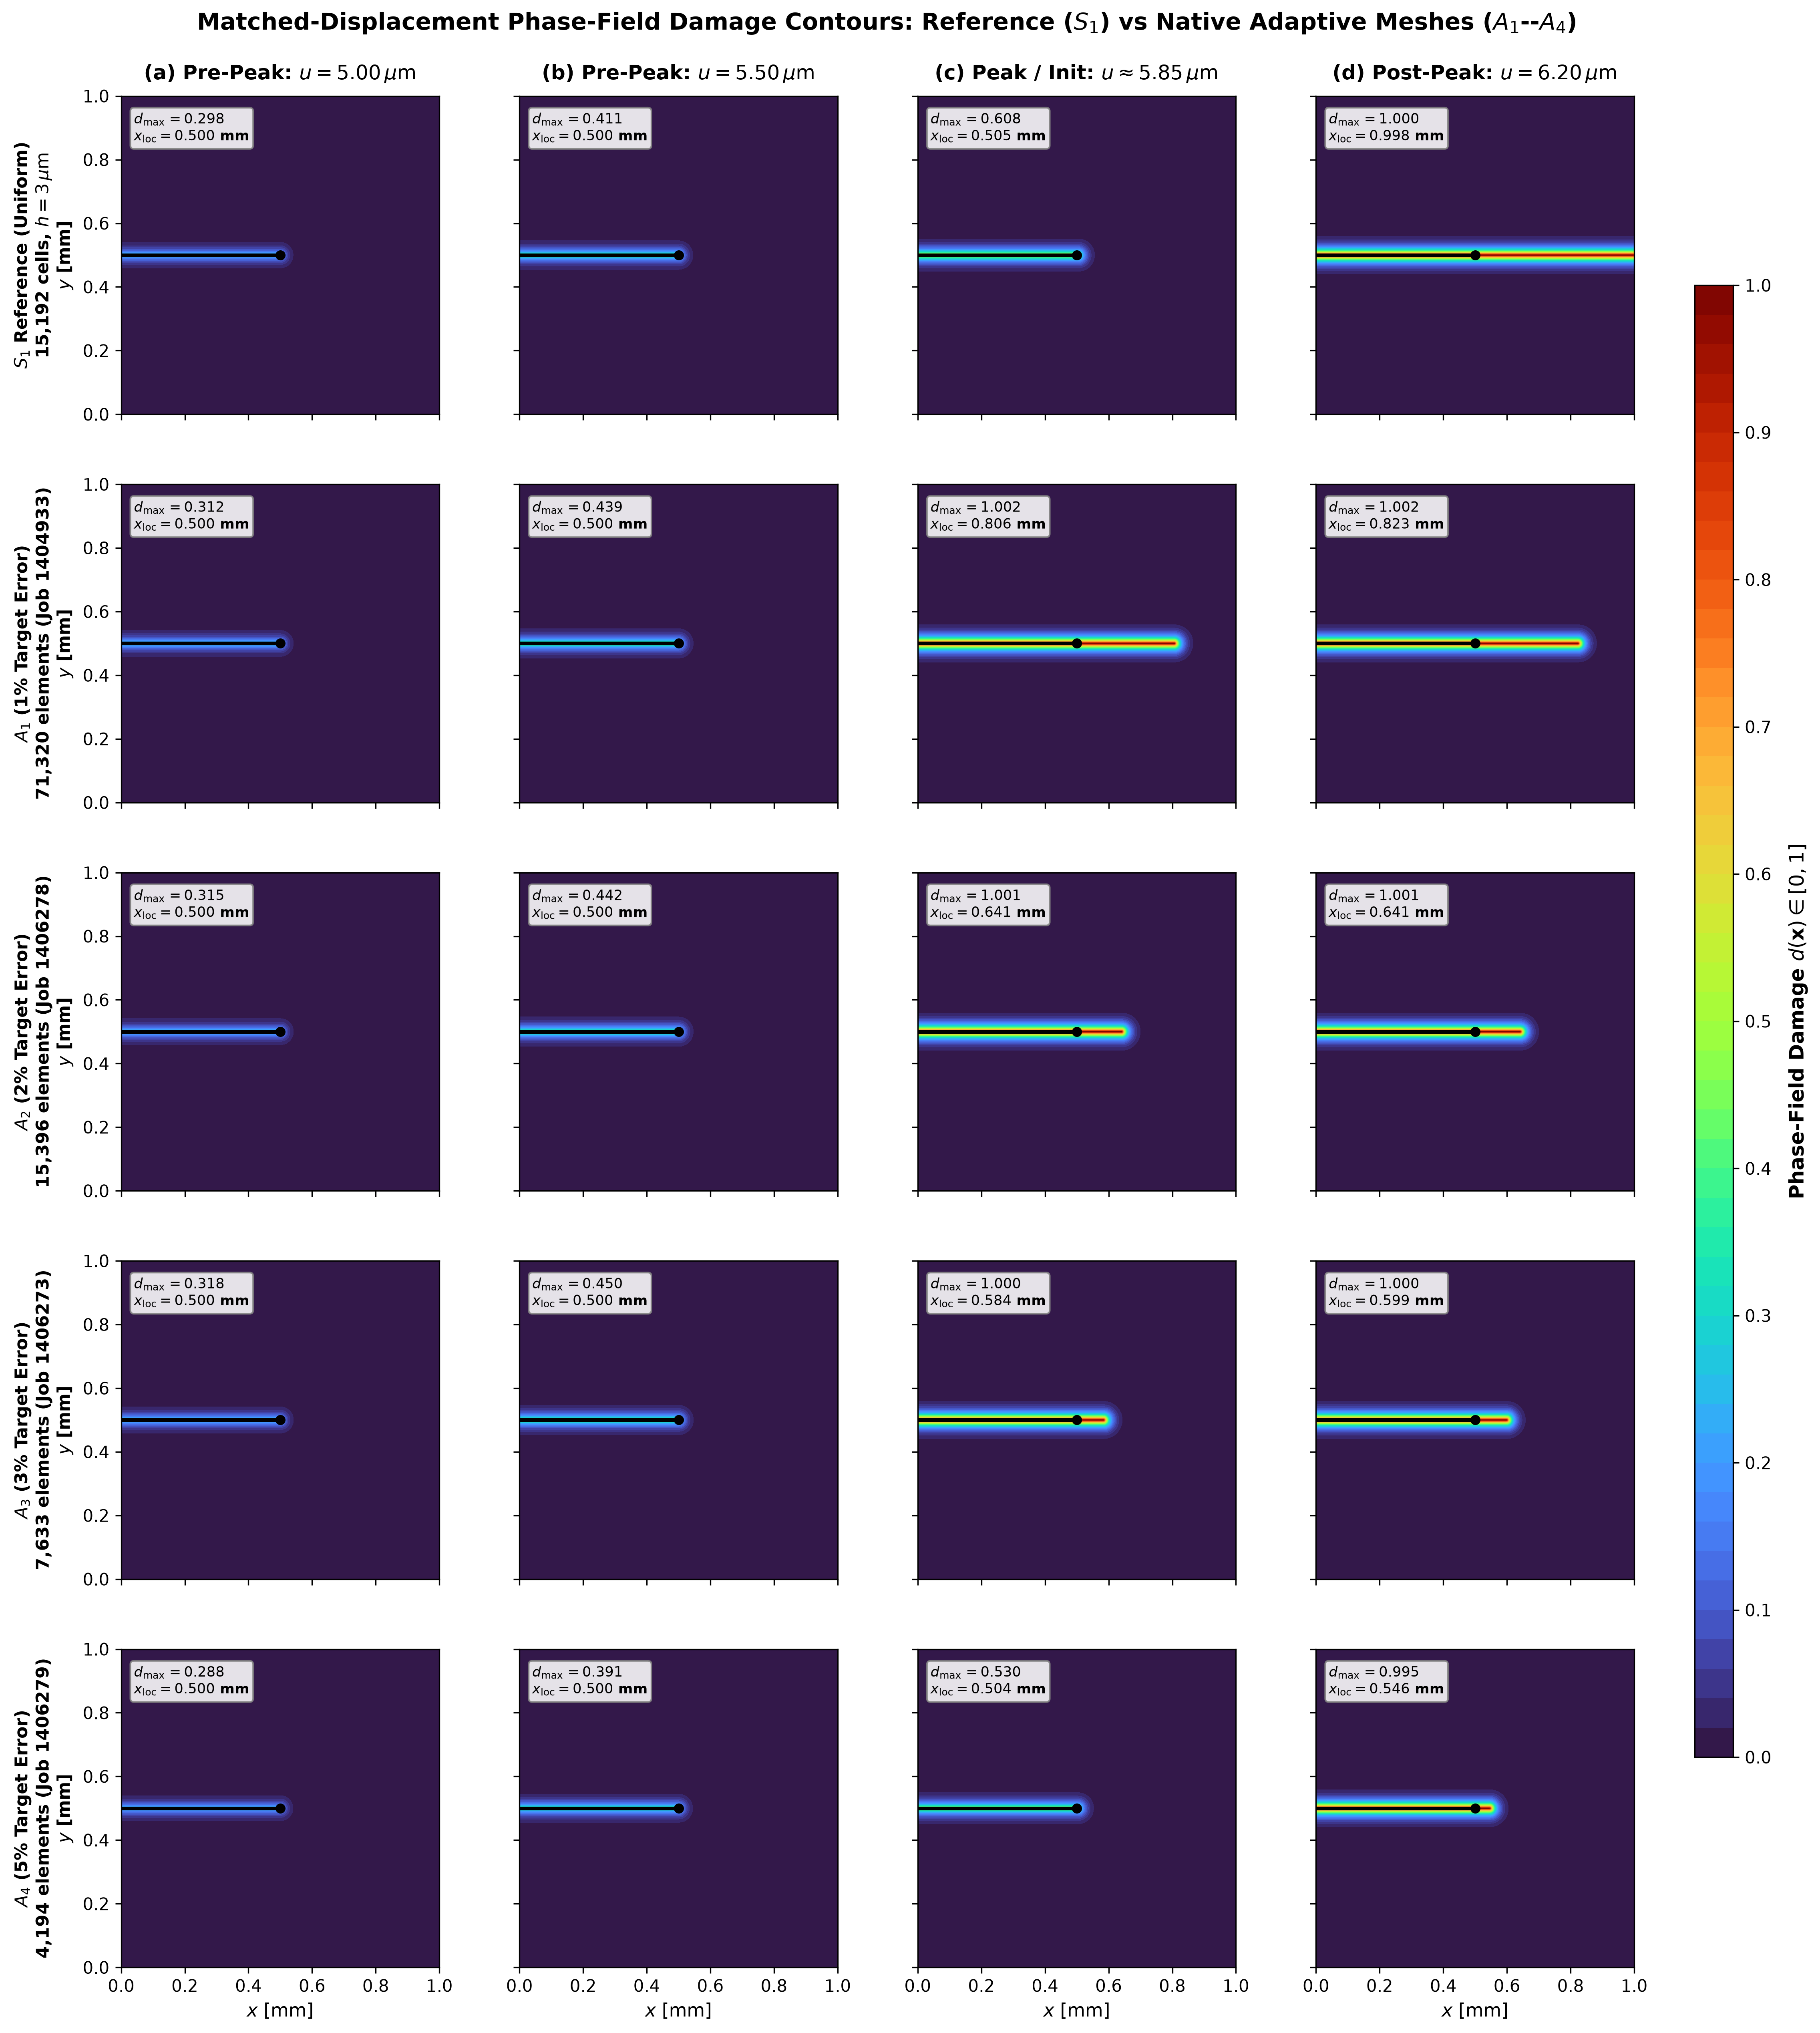
\includegraphics[width=0.88\textwidth]{gate6_matched_phase_field_contours.png}
  \caption{Matched-displacement phase-field damage contours comparing canonical reference $S_1$ ($15{,}192$ elements) and corrected native adaptive meshes $A_1$--$A_4$ across deformation states: (a) initiation at $u=5.00\,\mu\mathrm{m}$; (b) pre-peak concentration at $u=5.50\,\mu\mathrm{m}$; (c) peak / crack initiation at $u\approx 5.85\,\mu\mathrm{m}$; (d) post-peak propagated crack at $u=6.20\,\mu\mathrm{m}$.}
  \label{fig:matched_contours_pack}
  \figureconclusion{Pre-peak localization is broadly consistent, while crack-propagation timing and extent become resolution-dependent near and after the peak. The propagation direction nevertheless remains robustly aligned with the horizontal Mode-I path.}
\end{figure}

\begin{figure}[htbp]
  \centering
  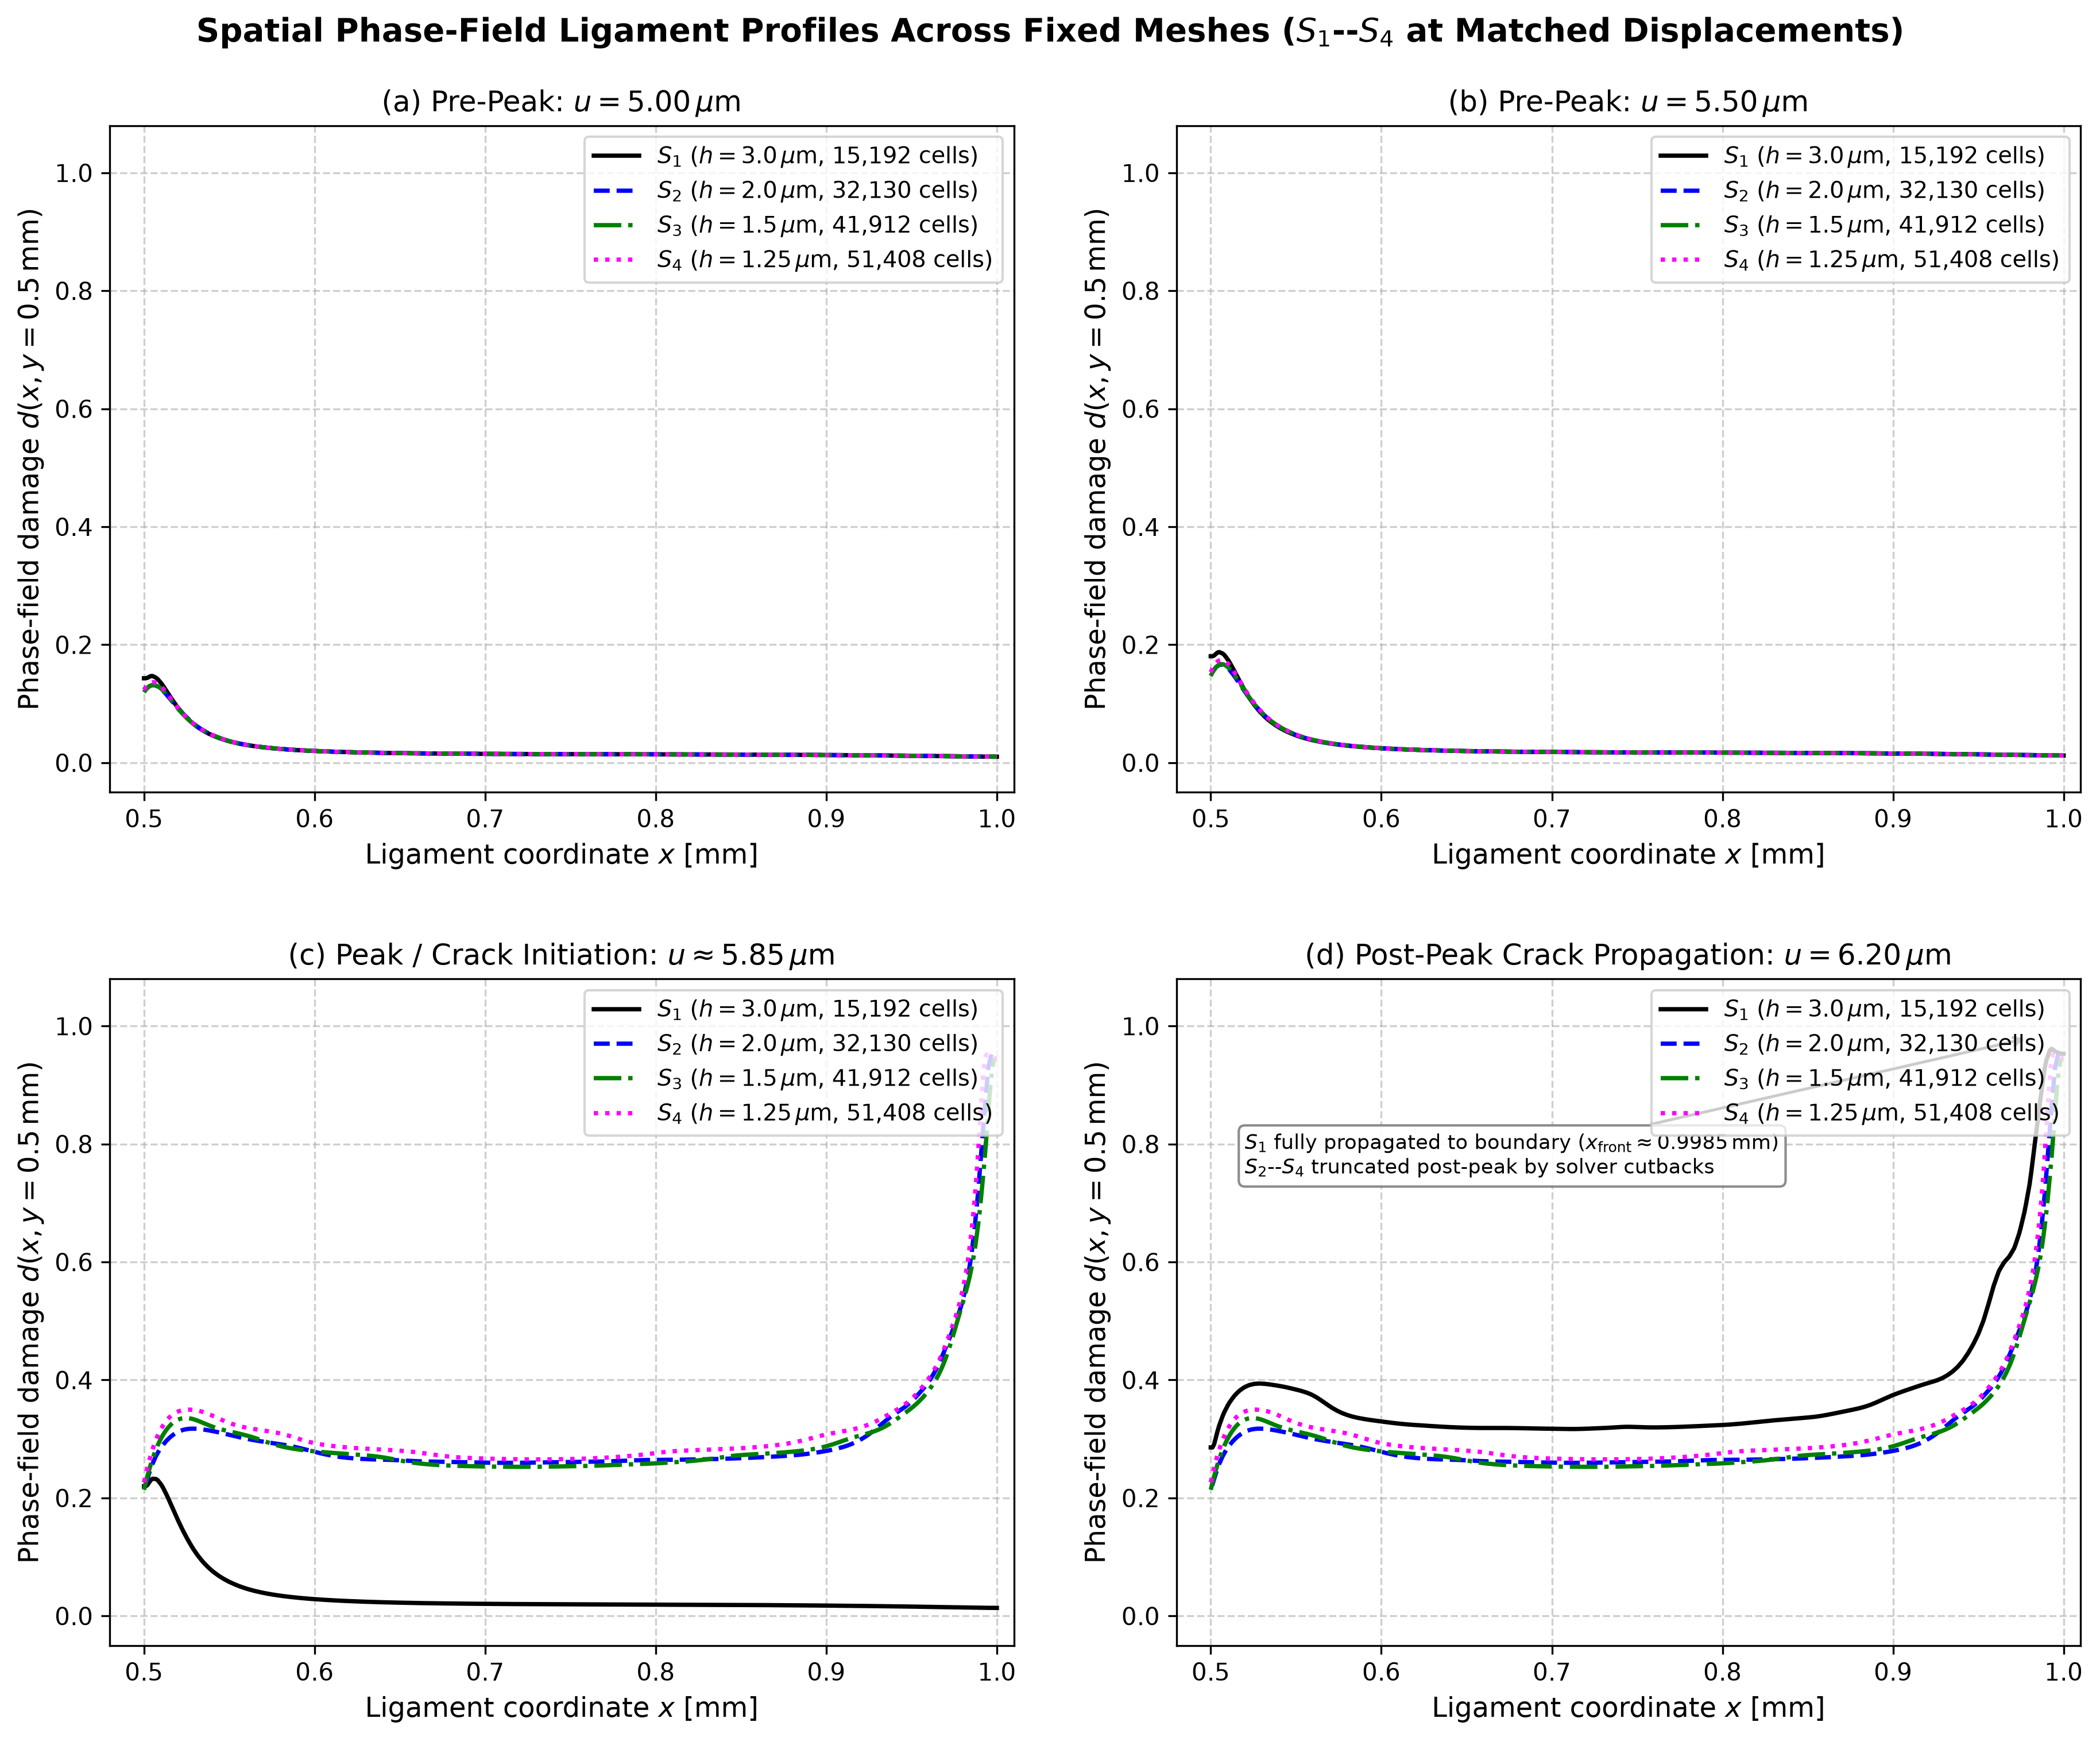
\includegraphics[width=0.88\textwidth]{fig1_fixed_mesh_ligament_profiles.png}
  \caption{Spatial phase-field ligament profiles $d(x, y=0.5\,\mathrm{mm})$ for fixed meshes $S_1$--$S_4$ across matched displacement levels, showing x-axis coordinates on all panels and annotating full boundary propagation in $S_1$ at $u = 6.20\,\mu\mathrm{m}$.}
  \label{fig:ligament_fixed_pack}
  \figureconclusion{Fixed meshes agree closely before peak loading. Near peak they separate because crack initiation occurs at different imposed displacements, and post-peak propagation extent differs; pre-peak localization is relatively stable, while near/post-peak evolution is mesh-sensitive.}
\end{figure}

\begin{figure}[htbp]
  \centering
  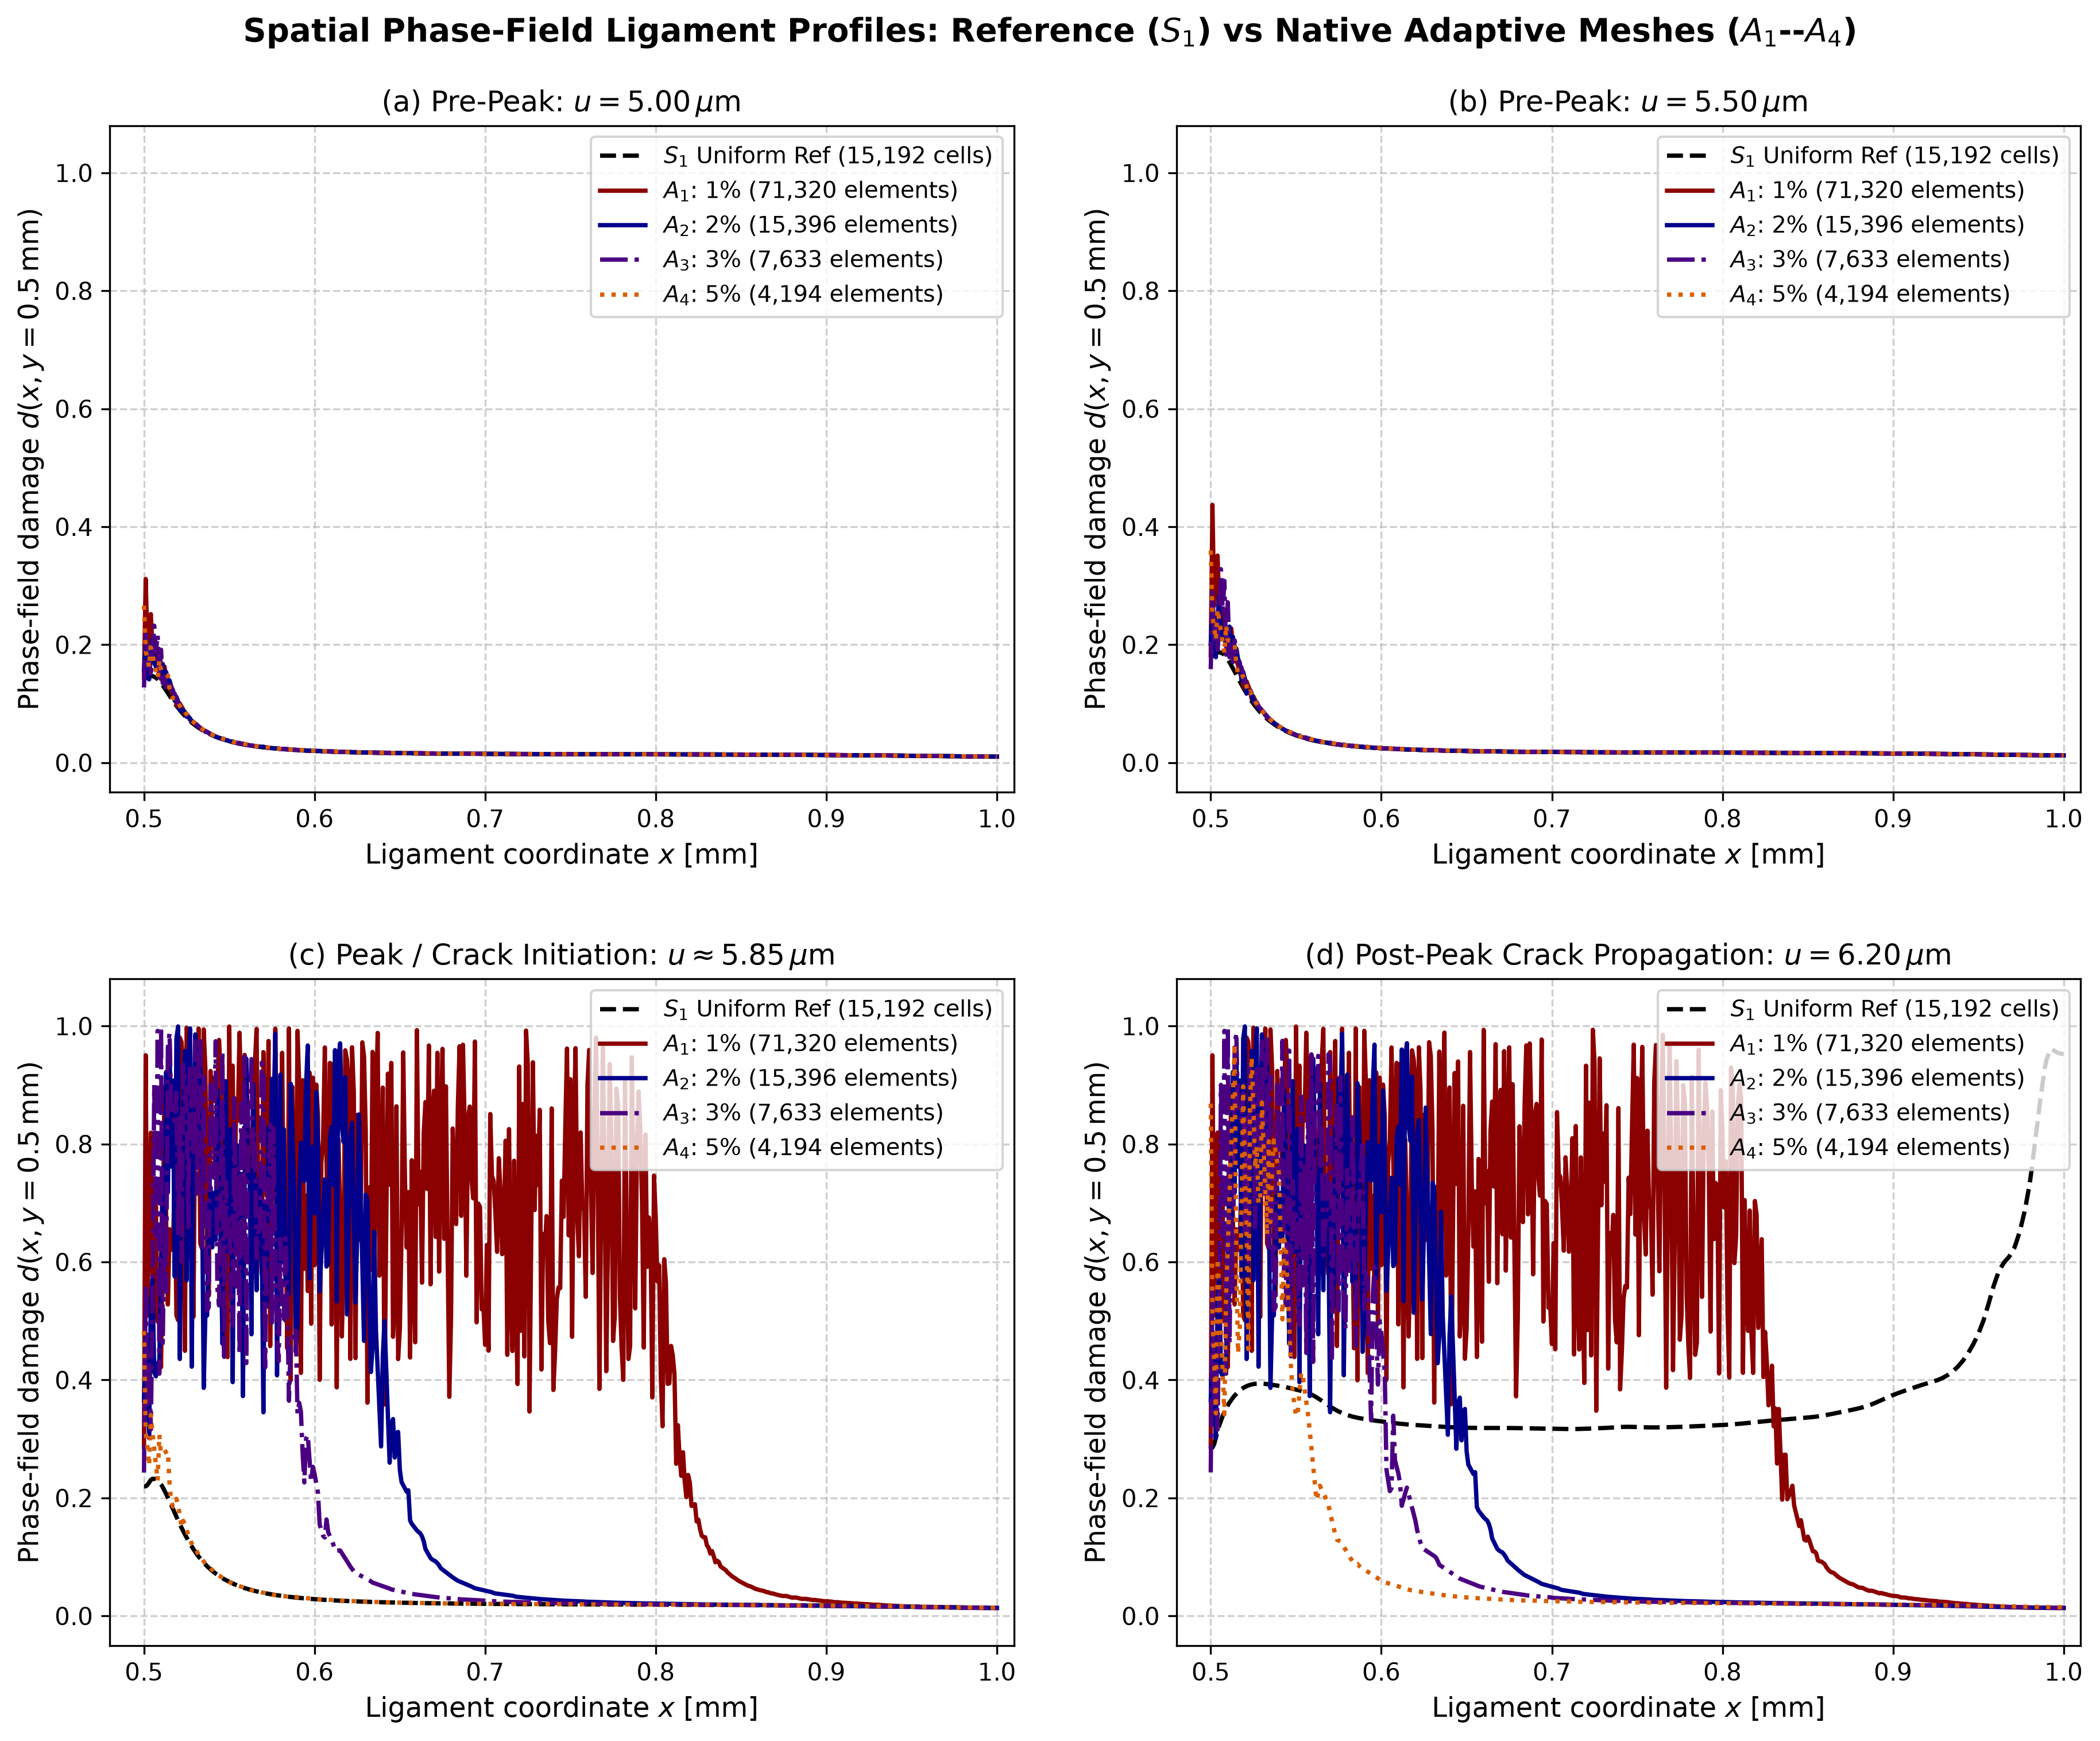
\includegraphics[width=0.88\textwidth]{fig2_adaptive_mesh_ligament_profiles.png}
  \caption{Spatial phase-field ligament profiles $d(x, y=0.5\,\mathrm{mm})$ comparing canonical reference $S_1$ against native adaptive meshes $A_1$--$A_4$ across matched displacement levels.}
  \label{fig:ligament_adaptive_pack}
  \figureconclusion{Adaptive pre-refinement reproduces the reference damage distribution reasonably well before the peak but diverges during crack initiation and unstable propagation. Post-peak crack evolution is therefore sensitive to the adaptive discretization.}
\end{figure}

\begin{figure}[htbp]
  \centering
  \includegraphics[width=0.92\textwidth]{fig_mode1_crack_propagation_sequence.pdf}
  \caption{Visual evolution of Mode-I crack propagation for the canonical $S_1$ reference baseline: six-stage sequence from initial elastic localization ($u = 5.0\,\mu\mathrm{m}$) through peak load ($u = 5.857\,\mu\mathrm{m}$) to complete ligament separation ($u = 6.20\,\mu\mathrm{m}$).}
  \label{fig:crack_sequence_pack}
  \figureconclusion{The canonical solution follows the expected Mode-I sequence: crack-tip localization, growth toward the limit load, initiation near the peak, rapid horizontal propagation, and complete ligament separation.}
\end{figure}

\begin{figure}[htbp]
  \centering
  \includegraphics[width=0.78\textwidth]{fig4_vertical_path_localization_deviation.png}
  \caption{Rigorous separation of (a) damage-weighted crack-centroid offset versus prescribed displacement ($|y_c - 0.5| \le 3.1\,\mu\mathrm{m}$, symmetric) and (b) damage localization-band half-width ($10$--$15\,\mu\mathrm{m}$, resolution-limited).}
  \label{fig:path_dev_pack}
  \figureconclusion{The crack trajectory remains essentially centered and is robustly Mode-I, whereas the thickness of the diffuse localization band remains resolution-sensitive. Crack direction and band width therefore exhibit different convergence behavior.}
\end{figure}

\clearpage

\subsection{Three-Point Physical Length-Scale Study ($l_0$ on Fixed $S_3$ Mesh)}
A controlled physical length-scale study was executed on the fixed $S_3$ mesh ($h = 1.5\,\mu\mathrm{m}$, $41{,}912$ finite elements, ensuring $h/l_0 \le 0.200$) across three regularization lengths $l_0 \in \{7.5, 11.25, 15.0\}\,\mu\mathrm{m}$ (Table~\ref{tab:l0_study_pack}, Fig.~\ref{fig:l0_metrics_pack}):
\begin{itemize}
  \item \textbf{Stiffness Invariance:} Initial structural stiffness $K_0$ varies from $137.857608$ to $137.676175\,\mathrm{kN/mm}$ ($\Delta = 0.13\%$), classified as \textbf{\texttt{INSENSITIVE / STABLE OVER TESTED RANGE}}.
  \item \textbf{Peak Force and Displacement Sensitivity:} Peak reaction force drops from $0.732196\,\mathrm{kN}$ ($l_0 = 7.5\,\mu\mathrm{m}$) to $0.689540\,\mathrm{kN}$ ($l_0 = 15.0\,\mu\mathrm{m}$, a $5.83\%$ reduction), while displacement at peak shifts from $5.633\,\mu\mathrm{m}$ to $5.579\,\mu\mathrm{m}$, classified as \textbf{\texttt{LENGTH-SCALE SENSITIVE}}.
  \item \textbf{Scope Limitation:} The $l_0 = 3.75\,\mu\mathrm{m}$ case ($h/l_0 = 0.400$) is excluded as under-resolved. Terminal energy comparison across the three cases is classified as \textbf{\texttt{NOT\_YET\_QUALIFIED\_UNEQUAL\_ENDPOINTS}}.
\end{itemize}

\begin{table}[htbp]
\centering
\caption{Three-point physical length-scale sensitivity metrics on fixed $S_3$ mesh ($h = 1.5\,\mu\mathrm{m}$).}
\label{tab:l0_study_pack}
\small
\begin{tabular}{lrrrrrr}
\toprule
$l_0$ [$\mu\mathrm{m}$] & Job ID & $h/l_0$ & Elements & $K_0$ [kN/mm] & $F_{\max}$ [kN] & $u_{\mathrm{peak}}$ [$\mu\mathrm{m}$] \\
\midrule
$7.50$ & \texttt{1406017.mmaster02} & $0.200$ & $41{,}912$ & $137.857608$ & $0.732196$ & $5.633$ \\
$11.25$ & \texttt{1406895.mmaster02} & $0.133$ & $41{,}912$ & $137.765563$ & $0.708402$ & $5.590$ \\
$15.00$ & \texttt{1406896.mmaster02} & $0.100$ & $41{,}912$ & $137.676175$ & $0.689540$ & $5.579$ \\
\bottomrule
\end{tabular}
\end{table}

\begin{figure}[htbp]
  \centering
  \begin{minipage}{0.48\textwidth}
    \centering
    \includegraphics[width=\textwidth]{fig_mode1_l0_fu_overlay.pdf}
    \caption*{(a) $F$--$u$ response across $l_0$}
  \end{minipage}\hfill
  \begin{minipage}{0.48\textwidth}
    \centering
    \includegraphics[width=\textwidth]{fig_mode1_l0_metrics_vs_lengthscale.pdf}
    \caption*{(b) Peak metrics vs.\ $l_0$}
  \end{minipage}
  \caption{Three-point physical length-scale study on fixed $S_3$ mesh ($h = 1.5\,\mu\mathrm{m}$): (a) global force-displacement overlay and (b) variation of $K_0$, $F_{\max}$, $u_{\mathrm{peak}}$, and matched $W_{\mathrm{trap}}$ at $u = 5.50\,\mu\mathrm{m}$ with $l_0$.}
  \label{fig:l0_metrics_pack}
  \figureconclusion{Changing $l_0$ leaves elastic stiffness nearly unchanged ($0.13\%$ spread) but materially lowers $F_{\max}$ and advances $u_{\mathrm{peak}}$. Elastic response is nearly length-scale-insensitive, while fracture initiation is physically length-scale-sensitive; terminal energies are not compared because endpoints differ.}
\end{figure}
